% В этом файле следует писать текст работы, разбивая его на
% разделы (section), подразделы (subsection) и, если нужно,
% главы (chapter).

% Предварительно следует указать необходимую информацию
% в файле SETUP.tex

%% В этот файл не предполагается вносить изменения

% В этом файле следует указать информацию о себе
% и выполняемой работе.

\documentclass [fontsize=14pt, paper=a4, pagesize, DIV=calc]%
{scrartcl}
% ВНИМАНИЕ! Для использования глав поменять
% scrartcl на scrreprt

% Здесь ничего не менять
\usepackage [T2A] {fontenc}   % Кириллица в PDF файле
\usepackage [utf8] {inputenc} % Кодировка текста: utf-8
\usepackage [russian] {babel} % Переносы, лигатуры

%%%%%%%%%%%%%%%%%%%%%%%%%%%%%%%%%%%%%%%%%%%%%%%%%%%%%%%%%%%%%%%%%%%%%%%%
% Создание макроса управления элементами, специфичными
% для вида работы (курс., бак., маг.)
% Здесь ничего не менять:
\usepackage{ifthen}
\newcounter{worktype}
\newcommand{\typeOfWork}[1]
{
	\setcounter{worktype}{#1}
}

% ВНИМАНИЕ!
% Укажите тип работы: 0 - курсовая, 1 - бак., 2 - маг.,
% 3 - бакалаврская с главами.
\typeOfWork{1}
% Считается, что курсовая и бак. бьются на разделы (section) и
% подразделы (subsection), а маг. — на главы (chapter), разделы и
%  подразделы. Если хочется,
% чтобы бак. была с главами (например, если она большая),
% надо выбрать опцию 3.

% Если при выборе 2 или 3 вы забудете поменять класс
% документа на scrreprt (см. выше, в самом начале),
% то получите ошибку:
% ./aux/appearance.tex:52: Package scrbase Error: unknown option ` chapterprefix=

%%%%%%%%%%%%%%%%%%%%%%%%%%%%%%%%%%%%%%%%%%%%%%%%%%%%%%%%%%%%%%%%%%%%%%%%
% Информация об авторе и работе для титульной страницы

\usepackage {titling}

% Имя автора #ИСПРАВИТЬ!
\newcommand {\byme}{%
\textbf{Ивахненко~Дмитрий~Игоревич}%
}

% Научный руководитель #ИСПРАВИТЬ!
\newcommand{\supervisor}%
{к.ф.-м.н., ст.преп. М. В. Юрушкин}



% Год публикации
\date{2020}

% Название работы #ИСПРАВИТЬ!
\title{\textbf{Семантический анализ фотографий с помощью глубоких нейронных сетей}}

% Кафедра
%

\newcommand {\direction} {%
02.\ifthenelse{\value{worktype} = 2}{04}{03}.02 --- Фундаментальная информатика и информационные технологии%
}

% Заведующий кафедрой #ИСПРАВИТЬ!
\newcommand{\headOfDepartment}{Штейнберг Б.\,Я.}

% Кафедра #ИСПРАВИТЬ!
\newcommand{\department}{Кафедра алгебры и дискретной математики}

%%%%%%%%%%%%%%%%%%%%%%%%%%%%%%%%%%%%%%%%%%%%%%%%%%%%%%%%%%%%%%%%%%%%%%%%
% Другие настраиваемые элементы текста

% Листинги с исходным кодом программ: укажите язык программирования
\usepackage{listings}
\lstset{
    language=[ISO]C++,%  Язык указать здесь
    basicstyle=\small\ttfamily,
    breaklines=true,%
    showstringspaces=false%
    inputencoding=utf8x%
}
% полный список языков, поддерживаемых данным пакетом, есть,
% например, здесь (стр. 13):
% ftp://ftp.tex.ac.uk/tex-archive/macros/latex/contrib/listings/listings.pdf

% Нумерация списков: можно при необходимести
% изменять вид нумерации (например, добавлять правую скобку).
% По умолчанию буду списки вида:
% 1.
% 2.
% Изменять вид нумерации можно в начале нумерации:
% \begin{enumerate}[1)] (В квадратных скобках указан желаемый вид)
\usepackage[shortlabels]{enumitem}
                    \setlist[enumerate, 1]{1.}

% Гиперссылки: настройте внешний вид ссылок
\usepackage%
[pdftex,unicode,pdfborder={0 0 0},draft=false,%backref=page,
    hidelinks, % убрать, если хочется видеть ссылки: это
               % удобно в PDF файле, но не должно появиться на печати
    bookmarks=true,bookmarksnumbered=false,bookmarksopen=false]%
{hyperref}


\usepackage {amsmath}      % Больше математики
\usepackage {amssymb}
\usepackage {textcase}     % Преобразование к верхнему регистру
\usepackage {indentfirst}  % Красная строка первого абзаца в разделе

\usepackage {fancyvrb}     % Листинги: определяем своё окружение Verb
\DefineVerbatimEnvironment% с уменьшенным шрифтом
	{Verb}{Verbatim}
	{fontsize=\small}

% Вставка рисунков
\usepackage {graphicx}

% Общее оформление
% ----------------------------------------------------------------
% Настройка внешнего вида

%%% Шрифты

% если закомментировать всё — консервативная гарнитура Computer Modern
\usepackage{paratype} % профессиональные свободные шрифты
%\usepackage {droid}  % неплохие свободные шрифты от Google
%\usepackage{mathptmx}
%\usepackage {mmasym}
%\usepackage {psfonts}
%\usepackage{lmodern}
%var1: lh additions for bold concrete fonts
%\usepackage{lh-t2axccr}
%var2: the package below could be covered with fd-files
%\usepackage{lh-t2accr}
%\usepackage {pscyr}

% Геометрия текста

\usepackage{setspace}       % Межстрочный интервал
\onehalfspacing

\newlength\MyIndent
\setlength\MyIndent{1.25cm}
\setlength{\parindent}{\MyIndent} % Абзацный отступ
\frenchspacing            % Отключение лишних отступов после точек
\KOMAoptions{%
    DIV=calc,         % Пересчёт геометрии
    numbers=endperiod % точки после номеров разделов
}

                            % Консервативный вариант:
%\usepackage                % ручное задание геометрии
%[%                         % (не рекомендуется в проф. типографии)
%  margin = 2.5cm,
  %includefoot,
  %footskip = 1cm
%] %
%  {geometry}

%%% Заголовки

\ifthenelse{\equal{\theworktype}{2}}{%
\KOMAoptions{%
    numbers=endperiod,% точки после номеров разделов
    headings=normal,   % размеры заголовков поменьше стандартных
    chapterprefix=true,% Печатать слово Глава в магистерской
    appendixprefix=true% Печатать слово Приложение
}
}

% шрифт для оформления глав и названия содержания
\newcommand{\SuperFont}{\Large\sffamily\bfseries}

% Заголовок главы
\ifthenelse{\value{worktype} > 1}{%
\renewcommand{\SuperFont}{\Large\normalfont\sffamily}
\newcommand{\CentSuperFont}{\centering\SuperFont}
\usepackage{fncychap}
\ChNameVar{\SuperFont}
\ChNumVar{\CentSuperFont}
\ChTitleVar{\CentSuperFont}
\ChNameUpperCase
\ChTitleUpperCase
}

% Заголовок (под)раздела с абзацного отступа
\addtokomafont{sectioning}{\hspace{\MyIndent}}

\renewcommand*{\captionformat}{~---~}
\renewcommand*{\figureformat}{Рисунок~\thefigure}

% Плавающие листинги
\usepackage{float}
\floatstyle{ruled}
\floatname{ListingEnv}{Листинг}
\newfloat{ListingEnv}{htbp}{lol}[section]

% точка после номера листинга
\makeatletter
\renewcommand\floatc@ruled[2]{{\@fs@cfont #1.} #2\par}
\makeatother


%%% Оглавление
\usepackage{tocloft}

% шрифт и положение заголовка
\ifthenelse{\value{worktype} > 1}{%
\renewcommand{\cfttoctitlefont}{\hfil\SuperFont\MakeUppercase}
}{
\renewcommand{\cfttoctitlefont}{\hfil\SuperFont}
}

% слово Глава
\usepackage{calc}
\ifthenelse{\value{worktype} > 1}{%
\renewcommand{\cftchappresnum}{Глава }
\addtolength{\cftchapnumwidth}{\widthof{Глава }}
}

% Очищаем оформление названий старших элементов в оглавлении
\ifthenelse{\value{worktype} > 1}{%
\renewcommand{\cftchapfont}{}
\renewcommand{\cftchappagefont}{}
}{
\renewcommand{\cftsecfont}{}
\renewcommand{\cftsecpagefont}{}
}

% Точки после верхних элементов оглавления
\renewcommand{\cftsecdotsep}{\cftdotsep}
%\newcommand{\cftchapdotsep}{\cftdotsep}

\ifthenelse{\value{worktype} > 1}{%
    \renewcommand{\cftchapaftersnum}{.}
}{}
\renewcommand{\cftsecaftersnum}{.}
\renewcommand{\cftsubsecaftersnum}{.}
\renewcommand{\cftsubsubsecaftersnum}{.}

%%% Списки (enumitem)

\usepackage {enumitem}      % Списки с настройкой отступов
\setlist %
{ %
  leftmargin = \parindent, itemsep=.5ex, topsep=.4ex
} %

% По ГОСТу нумерация должны быть буквами: а, б...
%\makeatletter
%    \AddEnumerateCounter{\asbuk}{\@asbuk}{м)}
%\makeatother
%\renewcommand{\labelenumi}{\asbuk{enumi})}
%\renewcommand{\labelenumii}{\arabic{enumii})}

%%% Таблицы: выбрать более подходящие

\usepackage{booktabs} % считаются наиболее профессионально выполненными
%\usepackage{ltablex}
%\newcolumntype {L} {>{---}l}

%%% Библиография

\usepackage{csquotes}        % Оформление списка литературы
\usepackage[
  backend=biber,
  hyperref=auto,
  sorting=none, % сортировка в порядке встречаемости ссылок
  language=auto,
  citestyle=gost-numeric,
  bibstyle=gost-numeric
]{biblatex}
\addbibresource{biblio.bib} % Файл с лит.источниками

% Настройка величины отступа в списке
\ifthenelse{\value{worktype} < 2}{%
\defbibenvironment{bibliography}
  {\list
     {\printtext[labelnumberwidth]{%
    \printfield{prefixnumber}%
    \printfield{labelnumber}}}
     {\setlength{\labelwidth}{\labelnumberwidth}%
      \setlength{\leftmargin}{\labelwidth}%
      \setlength{\labelsep}{\dimexpr\MyIndent-\labelwidth\relax}% <----- default is \biblabelsep
      \addtolength{\leftmargin}{\labelsep}%
      \setlength{\itemsep}{\bibitemsep}%
      \setlength{\parsep}{\bibparsep}}%
      \renewcommand*{\makelabel}[1]{\hss##1}}
  {\endlist}
  {\item}
}{}

% ----------------------------------------------------------------
% Настройка переносов и разрывов страниц

\binoppenalty = 10000      % Запрет переносов строк в формулах
\relpenalty = 10000        %

\sloppy                    % Не выходить за границы бокса
%\tolerance = 400          % или более точно
\clubpenalty = 10000       % Запрет разрывов страниц после первой
\widowpenalty = 10000      % и перед предпоследней строкой абзаца

% ----------------------------


% Стили для окружений типа Определение, Теорема...
% Оформление теорем (ntheorem)

\usepackage [thmmarks, amsmath] {ntheorem}
\theorempreskipamount 0.6cm

\theoremstyle {plain} %
\theoremheaderfont {\normalfont \bfseries} %
\theorembodyfont {\slshape} %
\theoremsymbol {\ensuremath {_\Box}} %
\theoremseparator {:} %
\newtheorem {mystatement} {Утверждение} [section] %
\newtheorem {mylemma} {Лемма} [section] %
\newtheorem {mycorollary} {Следствие} [section] %

\theoremstyle {nonumberplain} %
\theoremseparator {.} %
\theoremsymbol {\ensuremath {_\diamondsuit}} %
\newtheorem {mydefinition} {Определение} %

\theoremstyle {plain} %
\theoremheaderfont {\normalfont \bfseries} 
\theorembodyfont {\normalfont} 
%\theoremsymbol {\ensuremath {_\Box}} %
\theoremseparator {.} %
\newtheorem {mytask} {Задача} [section]%
\renewcommand{\themytask}{\arabic{mytask}}

\theoremheaderfont {\scshape} %
\theorembodyfont {\upshape} %
\theoremstyle {nonumberplain} %
\theoremseparator {} %
\theoremsymbol {\rule {1ex} {1ex}} %
\newtheorem {myproof} {Доказательство} %

\theorembodyfont {\upshape} %
%\theoremindent 0.5cm
\theoremstyle {nonumberbreak} \theoremseparator {\\} %
\theoremsymbol {\ensuremath {\ast}} %
\newtheorem {myexample} {Пример} %
\newtheorem {myexamples} {Примеры} %

\theoremheaderfont {\itshape} %
\theorembodyfont {\upshape} %
\theoremstyle {nonumberplain} %
\theoremseparator {:} %
\theoremsymbol {\ensuremath {_\triangle}} %
\newtheorem {myremark} {Замечание} %
\theoremstyle {nonumberbreak} %
\newtheorem {myremarks} {Замечания} %


% Титульный лист
% Макросы настройки титульной страницы
% В этот файл не предполагается вносить изменения

%\usepackage {showframe}

% Вертикальные отступы на титульной странице
\newcommand{\vgap}{\vspace{16pt}}

% Помещение города и даты в нижний колонтитул
\usepackage{scrlayer}
\DeclareNewLayer[
  foot,
  foreground,
  contents={%
    \raisebox{\dp\strutbox}[\layerheight][0pt]{%
      \parbox[b]{\layerwidth}{\centering Ростов-на-Дону\\ \thedate%
       \\\mbox{}
       }}%
  }
]{titlepage.foot.fg}
\DeclareNewPageStyleByLayers{titlepage}{titlepage.foot.fg}


\AtBeginDocument %
{ %
  %
  \begin{titlepage}
  %
    \thispagestyle{titlepage}

    {\centering
    %
    \MakeTextUppercase {МИНОБРНАУКИ РОССИИ}

    \vgap

    Федеральное государственное автономное образовательное\\
    учреждение высшего образования\\
    \textquote{Южный федеральный университет}

    \vgap

	Институт математики, механики \\ и компьютерных наук
    имени~И.\,И.\,Воровича

    \vgap
    
    \department
    
    \vgap
    \vgap
    
    \byme
    
    \vgap
    \vgap
    
    \MakeTextUppercase{\thetitle}
    
    \vgap
    \vgap

    \MakeTextUppercase{Выпускная квалификационная работа} \\ 
    по направлению подготовки \\
    \direction
    

    \vgap
    \vgap
    
    \textbf{Научный руководитель} -- \\
    \supervisor
    
    \vspace {\fill}
    
\ifthenelse{\value{worktype} = 1 \OR \value{worktype} = 3}{

\begin{flushleft}
    Допущено к защите:\\
    заведующий кафедрой \underline{\hspace{7cm}}\headOfDepartment
\end{flushleft}
}{}


  	\vspace {\fill}
  %Ростов-на-Дону

    %\thedate

  }\end{titlepage}
  %
  %
  \tableofcontents
  %
  \clearpage
} %


% Команды для использования в тексте работы


% макросы для начала введения и заключения
\newcommand{\Intro}{\addsec{Введение}}
\ifthenelse{\value{worktype} > 1}{%
    \renewcommand{\Intro}{\addchap{Введение}}%
}

\newcommand{\Conc}{\addsec{Заключение}}
\ifthenelse{\value{worktype} > 1}{%
    \renewcommand{\Conc}{\addchap{Заключение}}%
}

% Правильные значки для нестрогих неравенств и пустого множества
\renewcommand {\le} {\leqslant}
\renewcommand {\ge} {\geqslant}
\renewcommand {\emptyset} {\varnothing}

% N ажурное: натуральные числа
\newcommand {\N} {\ensuremath{\mathbb N}}

% значок С++ — используйте команду \cpp
\newcommand{\cpp}{%
C\nolinebreak\hspace{-.05em}%
\raisebox{.2ex}{+}\nolinebreak\hspace{-.10em}%
\raisebox{.2ex}{+}%
}

% Неразрывный дефис, который допускает перенос внутри слов,
% типа жёлто-синий: нужно писать жёлто"/синий.
\makeatletter
    \defineshorthand[russian]{"/}{\mbox{-}\bbl@allowhyphens}
\makeatother


\endinput

% Конец файла


\begin{document}

\Intro

В рамках данной работы освещается вопрос семантического анализа изображений путем применения глубоких сверточных нейронных сетей. Под семантическим анализом понимается получение из изображения какой-либо интерпретируемой информации: расположение объектов на сцене, принадлежность объектов к заранее заданным классам, наличие на изображении объектов определенного типа и т.п.. Данная тема будет рассмотрена на примере задачи обнаружения и выделения неба на изображениях. Входными данными задачи являются фотографии, сделанные на камеры мобильных устройств. Специализированный домен изображений был выбран с целью упрощения адаптация потенциального решения к применению в конечных продуктах, таких как пользовательское программное обеспечение для смартфонов. Решением задачи выступают сгенерированные для входных фотографий полутоновые изображения. Такое изображение называется сегментационной маской и для каждого пикселя исходной фотографии выражает его принадлежность к региону неба: белый цвет интерпретируется как положительный результат, черный - как отрицательный. В ходе разарботки алгоритма решения задачи была исселдована эффективность применения различных подходов к генерации подобного рода масок - сегментации. Сравнения эффективности проходило по индексу Жаккара - в западной литературе также встречается название intersection over union, IoU. Для решения задачи сегментации из наиболее эффективных подходов был составлен стек алгоритмов: применение к входному изображению глубокой сверточной сети с последующей корректировкой методами компьютерного зрения полученной маски. В ходе обучения модели искусственной нейронной сети, ИНС, для предотвращения переобучения и улучшения сходимости применялись техники регуляризация, такие как learning rate reduce и one cycle policy. Влияние данных подходов на решение также отражено в результатах работы. В заключительной части хода разработки была рассмотрена возможность адаптация модели, обученной на данных датасета SkyFinder, к выбранному домену изображений. Данная техника имеет название Domain Adaptation и используется для улучшения качества на практических данных.

% Если typeOfWork в SETUP.tex задан как 2 или 3, то начинать
% надо не с section (раздел), а с главы (chapter)
\section{Постановка и описание задачи}
\label{task_description_start}

Цифровая обработка изображений являются комплексной темой. В нее входят задачи фильтрации, цветовых и яркостных преобразований, морфологическая обработка, распознавание и выделение объектов на сцене~\autocite{gonzalez2008digital}. Семантический анализу - подход, целью которого является получение интерпретируемой информации высших порядков об изображении. К подзадачам семантического анализа можно отнести классификацию объектов на сцене, детекцию объектов и сегментацию изображений на семантические регионы. В рамках текущей работы будет проведен разбор подзадачи сегментации.

\subsection{Задача сегментации}

Для возможности цифровой обработки и анализа будем рассматривать представление изображения как трехмерного массива чисел, имеющего ширину, количество столбцов, и высоту, количество строк, равными ширине и высоте изображения соответсвенно. На каждой позиции по ширине и высоте будет находится вектор из трех целых чисел, из промежутка [0, 255], что соответсвует RGB модели представления цвета пикселя изображения. В таком случае сегментацией изображения будет являться отображение каждого RGB вектора в некоторое целое число. Это число соответствует идентификатору некоторого класса. При применение такого отображения ко всему изображению получается двумерный массив, ширина и высота которого соответсвуют таковым у исходного изображения. Подобный двумерный массив будет разделять изображение на регионы по обозначенному признаку и называться сегментационной маской. Сегментацию возможно рассматривать как попиксельную классификацию объектов.

\begin{figure}[H]
 \centering
 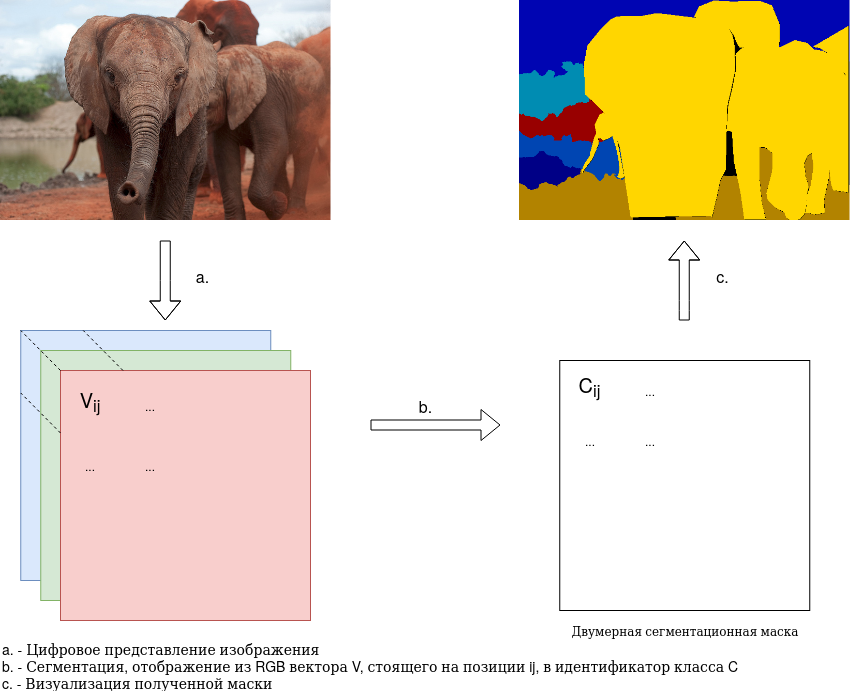
\includegraphics[width=\textwidth]{img/example_segmentation.png}
 \caption{Общий вид сегментации на примере данных датасета COCO}
 \label{fig:seg_example}
\end{figure}

Отметим, что описанное выше отображение может обладать относительно простой природой и учитывать только значение пикселя в конкретной позиции, так и более сложной структурой, использующей информацию о распределении цветов во всем изображении, положении пикселя на изображении и свойствах соседних пикселей, непосредственно соседствующих с обозреваемым значением или отсупающих от него на заданное смещение~\autocite{liu2018recent}. На \ref{fig:seg_example} показан общий вид задачи сегментации изображения.



\subsection{Выделение неба в рамках задачи сегментации}

Описанная в введение задача выделения региона неба на входном изображении может быть рассмотрена как задача сегментации. Так как в данном случае результирующих классов всегда два - класс принадлежности и обратный ему -, то имеется более узкий случай сегментации - бинарная. Итоговая маска будет содержать только значения 0 и 1, представляя собой однобитовое бинарное изображение, что можно считать вырожденным полутоновым.

Таким образом, решение задачи выделения неба сводится к нахождению отображения из вектора цветов для каждого пикселя в целое число из промежутка [0, 1]. Данное отображение возможно получить как алгоритмами машинного зрения, так и с помощью использования моделей глубоких сверточных нейронных сетей. В данной работе приводится решение методом нейронных сетей, при этом алгоритмы компьютерного зрения используются для корректировки полученной маски. Под корректировкой здесь понимается обнаружение и удаление ложноположительных регионов неба небольшой площади.

\begin{figure}[H]
 \centering
 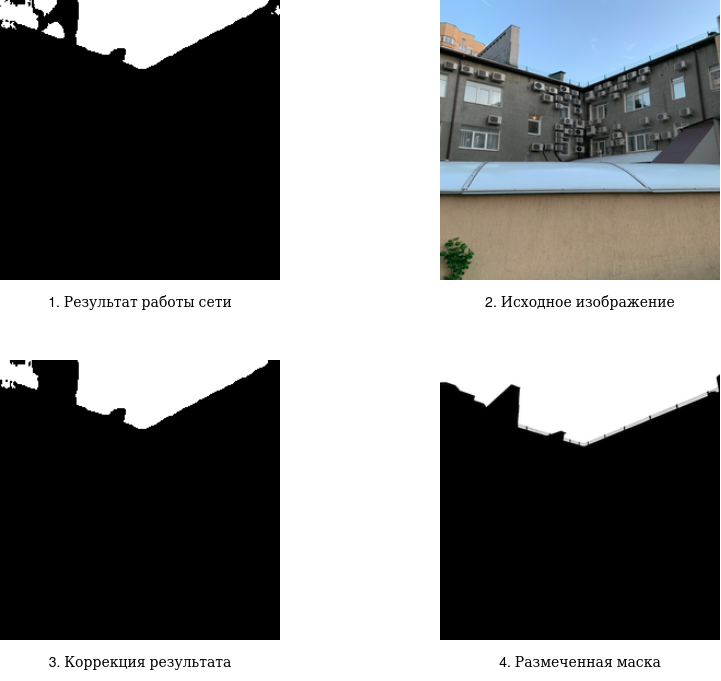
\includegraphics[width=\textwidth]{img/sky_segmentation.png}
 \caption{Пример, демонстрирующий работу алгоритма}
 \label{fig:sky_seg}
\end{figure}

Практическое применение подобного решения можно найти в пользовательских приложениях эстетической обработки пейзажных фотографий для смартфонов, в автоматических системах мониторинга воздушного пространства, при извлечении семантической информации высшего порядка для использования в иных методах анализа и обработки изображений~\autocite{7415405}.

\section{Обзор решений}

Задача семантического анализа изображений имеет широкое применение при решении различных прикладных и исследовательских проблем~\autocite{maier2018gentle}~\autocite{pan2019image}~\autocite{stabinger2020evaluating}~\autocite{li2015brief}, в связи с чем активно изучается. Сегментации изображений, в частности, нашли применения в таких областях как проведение хирургических операций, автопилотируемый транспорт, автоматизированное картографирование местности~\autocite{liu2018recent}. Ниже приведен краткий обзор исследований, темы которых связаны с поставленной задачей. Результаты этих исследований в разной степени использовались для построения решения. 

\subsection{Сегментация изображений}

До начала активного применения глубоких нейронных сетей в задачах сегментации использовались методы компьютерного зрения, основанные на применении порогов бинаризации для полутоновых изображений, выявлении признаков, кластеризации методом k-средних~\autocite{10.5555/1888028.1888043}~\autocite{10.5555/540298}~\autocite{inproceedings}. Каждый из этих подходов имеет свои приемущества, метод бинарной сегментации полутоновых изображений до сих пор успешно применяется в области анализа медицинских данных~\autocite{bookMedicalImages}. Но применение данных подходов к задаче выделения границы между объектами путем сегментации показало худшие результаты в сравнении с FCN, полностью сверточными глубокими сетями~\autocite{7966418}.

Современные решения задачи сегментации в различных областях зачастую опираются на применение нейронных сетей~\autocite{feng2019deep}. Наиболее распространенными архитектурами выступают Unet, DeepLab, RefineNet~\autocite{ronneberger2015unet}~\autocite{chen2016deeplab}~\autocite{lin2016refinenet}. Имеются исследования применения архитектуры RefineNet для определния региона неба на датасете SkyFinder~\autocite{place2017segmenting}.


\subsection{Методы регуляризации}

Помимо специализированных решений задачи сегментации, были рассмотрены также общие методики, применяемые для обучения глубоких нейронных сетей. При высокой сложности модели, в процессе обучения она может начать отражать в ответах шум в тренировачных данных~\autocite{salman2019overfitting}~\autocite{ghojogh2019theory}. Данное явление называется переобучением, overfitting. С целью снизить вероятность его проявление применяются разнообразные техники регуляризации: dropout, нормализация значений между слоями сети, настройка гиперпараметров процесса обучения~\autocite{smith2018disciplined}~\autocite{labach2019survey}~\autocite{ioffe2015batch}.

\section{Метод решения}

Конечное решение задачи сегментации имеет комплексное строение. Изображение, поступающее на вход решающему алгоритму, обрабатывается ИНС. Результатом такого применения является двумерный массив пар. Каждое значение в паре обозначет вероятность принадлежности одному из двух классов. Для получения сегментационной маски индекс максимального из двух значений расценивается как идентификатор класса: 1 для региона неба, 0 - обратный ему. В ходе экспериментов было выявлено наличие артефактов в результатах классификации. Для части изображений имелись ложноположительные регионы неба небольшой площади. Для их устранения последовательно применялись алгоритмы FindCounters и DrawCounters из состава библиотеки OpenCV. 

Для обучения сети использовался датасет SkyFinder. Для улчушения показателя IoU на целевом домене изображений использовалась техника Unsupervised Domain Adaptation. Это позволило уменшить количество ложноположительных и ложноотрицательных регионов без дополнительной разметки обучающий выборки из фотографий, сделанных на мобильные устройства.

\subsection{Глубокая сверточная сеть}

Как было отмечено выше, текущие исследования указывают на приемущества глубоких сверточных сетей в задачах семантического анализа перед классическими алгоритмами компьютерного зрения. Глубокими сверточными сетями называют подвид искуственных нейронных сетей, все слои которой являются сверточными. 

Архитекутра сети для решения задачи сегментации представляется двумя частями. Выделение признаков, downsampling path, и генерализация результатов выделения, upsampling path. Для решения проблемы потери информации в сверточных слоях, карты признаков с некоторых уровней нисходящей части объединяют с противополженными входами восходящей части.

В нисхоядщей части используются обычные сверточные слои, сверточные слои с выбором наибольшего значения по ядру - max pooling. На сверточных слоях к входным данным применяются ядра свертки. Количество ядер определяет для слоя количество выходных карт признаков. Выходные карты признаков подаются на вход следующему слою. К выходным картам применяется функция активации. Значения в ядрах свертки являются тренируемыми параметрами сети. Ниже приведена формула для простого случая двумерного входного массива и двумерного ядра свертки (\ref{eq:1}).

\begin{equation} 
\label{eq:1}
G[m, n] = (f*h)[m, n] = \sum_{j}{\sum_{k}{h[j, k]f[m + j, n + k]}}
\end{equation}

где f - входной массив данных, h - ядро свертки, G - выходная карта признаков.

Размеры каждой карты определяются размерами входных данных, размерами ядра, размером добавочного отступа по краям массива данных и сдвигом, на которое ядро смещается по массиву (\ref{eq:2}). 

\begin{equation}
\label{eq:2}
output = \frac{input + 2 * a - k}{s} + 1
\end{equation}

где output - размеры выходной карты признаков, input - размеры входного массива данных, a - величина отсутпа, добавляемого к краям массива, k - размеры ядра свертки, s - сдвиг ядра.

В сверточных слоях с выбором наибольшего значения ядро задает только размеры окна, в котором выбирается максимальный элемент. Операции сложения и умножения на этом слое не используются. 

\section{Данные}

Эксперименты с обучением модели ИНС проводились на двух наборах данных: SkyFinder и набор из фотографий, сделанных на камеры смартфонов, с синтетической разметкой в объединении с данными из SkyFinder. 

\subsection{Датасет SkyFinder}

SkyFinder представляет собой набор из 90.000 фотографий~\autocite{mihail2016sky}. Все фотографии сделаны на статичные веб-камеры, расположенные вне зданий. В верхней части изображений преобладает регион неба. Средний процент пикселей относящихся к классу принадлжености равен 41 со стандартным отклонением в 16 процентов. Изображения покрывают широкий диапозон освещенности и погодных условий, что препятсвует переобучению на конкретных значениях. Для каждого изображения имеется размеченная бинарная маска с описанным в постановке задачи свойством: 1 обозначает класс принадлежности, 0 - обратный ему. 

\subsection{Датасет с синтетической разметкой}



\Conc

% Печать списка литературы (библиографии)
\printbibliography[%{}
    heading=bibintoc%
    %,title=Библиография % если хочется это слово
]
% Файл со списком литературы: biblio.bib
% Подробно по оформлению библиографии:
% см. документацию к пакету biblatex-gost
% http://ctan.mirrorcatalogs.com/macros/latex/exptl/biblatex-contrib/biblatex-gost/doc/biblatex-gost.pdf
% и огромное количество примеров там же:
% http://mirror.macomnet.net/pub/CTAN/macros/latex/contrib/biblatex-contrib/biblatex-gost/doc/biblatex-gost-examples.pdf

\end{document}
